%!TEX root = ../ecdsa.tex

\chapter{Implementierung} \label{sec:impl}

%%%%%%%%%%%%%%%%%%%%%%%%%%%%%%%%%%%%%%%%%%%%%%%%%%%%%%%%%%%%%
\section{Architektur \& Moduldesign} 
\label{sec:march}
Die Architektur der VHDL-Implementierung verwendet einen modularen Ansatz. Die zentrale Komponente wird durch den Controller repräsentiert, der den Zustandsautomat, die ECC-, sowie die arithmetischen Operationen beinhaltet und damit die ECDSA-Funktionen (Signieren, Verifizieren)  implementiert. Abbildung \ref{fig:vhdl-impl-arch} zeigt den grundlegenden Aufbau des Systems.   

\begin{figure}[H]
	\centering
  	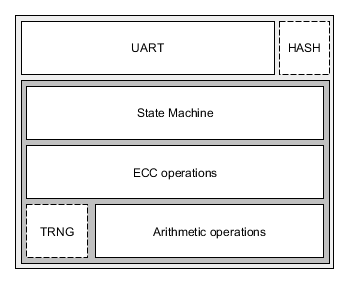
\includegraphics[width=0.7\textwidth]{bilder/vhdl_overview.png}
	\caption{Modulübersicht der FPGA-Hardware}
	\label{fig:vhdl-impl-arch}
\end{figure}
 
Die Umschaltung zwischen den verschiedenen Algorithmen findet über einen Zustandsautomat (engl. State Machine) statt. Die Hardware-Implementierung kann zwischen den Modi Signieren und Verifizieren unterschieden. Die Umschaltung findet über die UART-Schnittstelle statt, indem der Datenstrom analysiert wird. Eine detaillierte Beschreibung ist in Abschnitt \ref{sec:uartimpl} zu finden. Je nach gewünschter Funktion, werden andere Parameter über UART empfangen bzw. zurückgeschickt. Eine Übersicht der Parameter beinhaltet Tabelle \ref{tab:vhdl-impl-uart-data}. \\

\begin{table} [h]
	\centering 
	\begin{tabular}{ | p{3cm} | p{2cm} | p{6cm} | }
		\hline
		\textbf{Funktion} & \textbf{Typ} & \textbf{Parameter} \\
		\hline
		Signieren & Input &  Nachricht $m$ (163 Bit) \\
		\hline
		Signieren & Ouput & Signatur $(r,s)$ (326 Bit) \\
		\hline
		Verifizieren & Input & Nachricht $m$ (163 Bit) \\
		\hline
		Verifizieren & Input & Signatur $(r,s)$ (326 Bit) \\
		\hline
		Verifizieren & Output & Ergebnis der Verifizierung (1 Bit) \\
		\hline
	\end{tabular}
	\caption{Eingabe- und Ausgabedaten der VHDL-Implementierung}
	\label{tab:vhdl-impl-uart-data}
\end{table}
 
Wie bereits in Kapitel \ref{sec:planung} erwähnt, wurde auf eine sicherheitsorientierte Implementierung des Algorithmus verzichtet, sodass anstatt eines ``echten'' Zufallszahlengenerators  (engl. True Random Number Generator, TRNG), lediglich eine festgelegte Konstante zum Einsatz kommt. Hauptgrund für diese Entscheidung begründet sich mit der fehlenden Hardware zum Generieren einer sicheren Zufallszahl. Als eine weitere Vereinfachung wurde auf eine Einheit zum Generieren eines Hashes verzichtet, um den Fokus auf die Implementierung der ECC-Operationen zu lenken, ohne die Messergebnisse durch die HASH-Generierung zu verfälschen. Aus Gründen der Vollständigkeit sind beide Komponenten dennoch in Abbildung \ref{fig:vhdl-impl-arch} zu finden. 

%%%%%%%%%%%%%%%%%%%%%%%%%%%%%%%%%%%%%%%%%%%%%%%%%%%%%%%%%%%%%

\section{Parameter}
\label{vhdl-impl-parameter}

Die gesamte VHDL-Implementierung setzt ausschließlich auf VHDL-typische \texttt{Generics}. Diese werden über das globale Paket \texttt{tld\_ecdsa\_package} verwaltet. Neben den Parametern enthält das Paket globale Hilfsfunktionen, die zum Beispiel eine Matrix-Reduktion durchführen. Tabelle \ref{tab:vhdl-impl-param} zeigt eine Übersicht der wichtigsten Parameter.
\\ \\
Wie der Tabelle \ref{tab:vhdl-impl-param} zu entnehmen ist, sind in der Datei auch der private, der öffentliche Schlüssel und die k-Konstante  zu finden. Die Schlüssel wurden direkt als Konstanten hinterlegt, um die Kommunikation über die UART-Schnittstelle zu vereinfachen. Für den Einsatz der Software in einer produktiven Umgebung sollte  der öffentliche Schlüssel austauschbar sein, sodass auch Signaturen von Anderen verifiziert werden können. Das gleiche gilt für den privaten Schlüssel, um in der Lage zu sein, nachträglich die Schlüssel aus sicherheitsgründen auszutauschen oder allgemein Signaturen mit verschiedenen Schlüsseln zu erstellen.
\\ \\
Durch den Einsatz der generischen Implementierung ist es möglich, Parameter nachträglich zu ändern, um beispielsweise eine andere Schlüssellänge oder Kurvenparameter zu verwenden. Ein Nachteil dagegen ist, dass durch die generische Implementierung weniger Spielraum für Performanz-Optimierungen besteht. Da mit wachsender Leistungsfähigkeit heutiger Systeme aber auch die Anforderung an kryptografische steigt, wurde die nachträgliche Anpassbarkeit der Parameter als wichtiger angesehen. \\

\begin{table} [h]
	\centering 
	\begin{tabular}{ | p{3cm} | p{12cm} | }
		\hline
		\textbf{Parameter} & \textbf{Beschreibung}\\
		\hline
		M & Bitbreite des Schlüssels bzw. der Daten (z.B. 163) \\
		\hline
		N & Modulo-Parameter der Kurve (Bestandteil des ECDSA-Algorithmus) \\
		\hline
		A & A-Parameter der Kurve (Bestandteil des ECDSA-Algorithmus) \\
		\hline
		P & Anzahl der Elemente im GF($2^M$) \\
		\hline
		xG & x-Komponenten des Generator-Punktes \\
		\hline
		yG & y-Komponenten des Generator-Punktes \\
		\hline
		dA & Privater Schlüssel für die Signierung \\
		\hline
		xQ & x-Komponenten des öffentlichen Schlüssel für die Verifizierung \\
		\hline
		yQ & y-Komponenten des öffentlichen Schlüssel für die Verifizierung \\
		\hline
		k & (statische) Zufallszahl \\
		\hline
		BAUD\_RATE & Eingestellte Baud-Rate der UART-Schnittstelle \\
		\hline
	\end{tabular}
	\caption{Parameter der VHDL-Implementierung}
	\label{tab:vhdl-impl-param}
\end{table}


%%%%%%%%%%%%%%%%%%%%%%%%%%%%%%%%%%%%%%%%%%%%%%%%%%%%%%%%%%%%%

\section{Top-Level-Entität}
\label{vhdl-impl-tld}

Wie bereits erwähnt kommuniziert die Top-Level-Entität über eine serielle RS232-Schnittstelle mit einem Computer, um Daten auszutauschen. Dazu werden lediglich zwei Pins zur UART-Kommunikation, sowie ein globales 50Mhz-Takt- und ein Resetsignal benötigt. Tabelle \ref{tab:vhdl-impl-tld-ecdsa-param} beschreibt die Parameter der Entität. \\

\begin{figure}[thb]
	\centering
	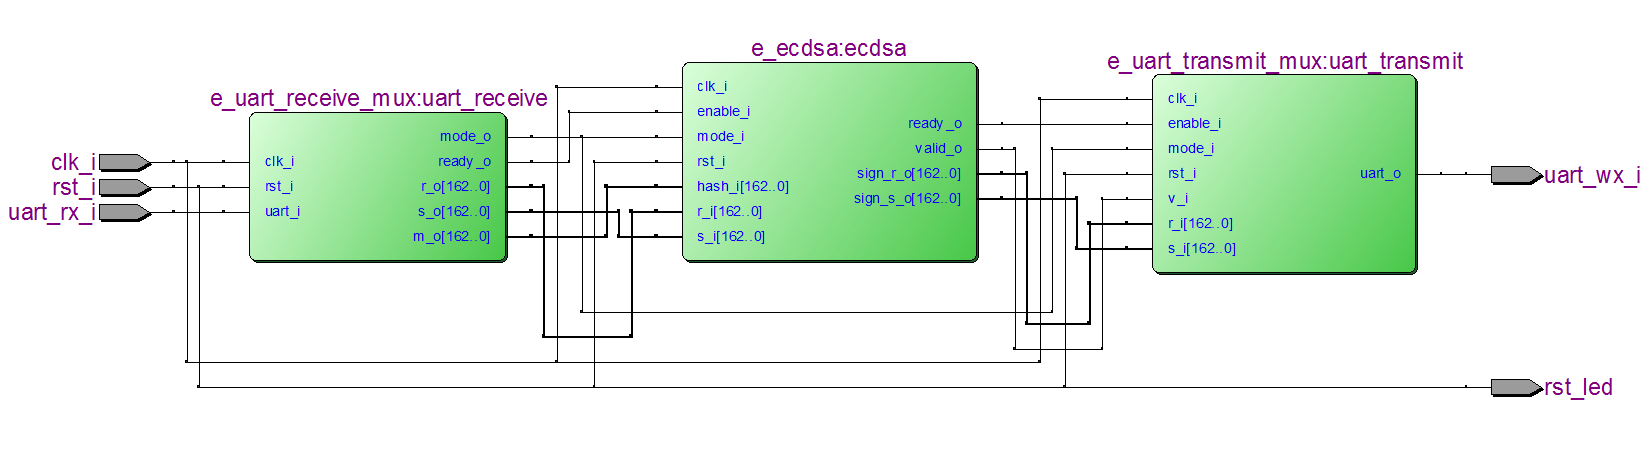
\includegraphics[width=\textwidth]{bilder/tle}
	\caption{Top-Level-Entity der VHDL-Implementierung}
	\label{fig:vhdl-impl-tle}
\end{figure}

Nach vollständigem Erhalt der Daten, die sich je nach Algorithmus unterscheiden (vgl. Tabelle \ref{tab:vhdl-impl-uart-data}), werden diese dem zentralen Modul \texttt{e\_ecdsa} bereitgestellt. Über binäre Eingänge wird festgelegt, welcher Modus (Signieren vs. Verifizieren, Pin \texttt{mode\_i}) verwendet und wann die Berechnung gestartet werden soll (Pin \texttt{enable\_i}). Sobald die ECDSA-Entität die Berechnung abgeschlossen hat, wird ein binäres Flag gesetzt, sodass die Daten über das Modul \texttt{e\_uart\_transmit\_mux} zurückschickt werden können. \\
 
\begin{table} [h]
	\centering 
	\begin{tabular}{ | p{3cm} | p{12cm} | }
		\hline
		\textbf{Parameter} & \textbf{Beschreibung}\\
		\hline
		clk\_i & Globales Taktsignal \\
		\hline
		rst\_i & Resetsignal \\
		\hline
		uart\_rx\_i & Pin zum Lesen der UART-Kommunikation \\
		\hline
		uart\_tx\_i & Pin zum Schreiben der UART-Kommunikation \\
		\hline
		rst\_led & LED zur Kennzeichnung ob das Reset-Signal aktiv ist \\
		\hline
	\end{tabular}
	\caption{Eingabe- und Ausgabeparameter der Haupt-Entität}
	\label{tab:vhdl-impl-tld-ecdsa-param}
\end{table} 


%%%%%%%%%%%%%%%%%%%%%%%%%%%%%%%%%%%%%%%%%%%%%%%%%%%%%%%%%%%%%
\section{ECDSA-Implementierung}
\label{vhdl-impl-general}

\subsection{Allgemeiner Aufbau der VHDL-Entitäten}
\label{vhdl-impl-general-entity}

Jede Entität, sei es eine mathematische oder eine zusammengesetzte Komponente wie die ECC-Operationen, verwendet den selben Aufbau. So besitzen die Entitäten neben einem globalen Takt- und Resetsignal ein Aktivierungs- und ein Status-Flag, sowie eine beliebige Anzahl anwendungsabhängiger Eingabe- bzw. Ausgabeparameter. Eine Übersicht der Parameter ist in Tabelle \ref{tab:vhdl-impl-ecdsa-general} zu finden. \\

\begin{table} [h]
	\centering 
	\begin{tabular}{ | p{3cm} | p{12cm} | }
		\hline
		\textbf{Parameter} & \textbf{Beschreibung}\\
		\hline
		clk\_i & Globales Taktsignal \\
		\hline
		rst\_i & Resetsignal \\
		\hline
		enable\_i & Flag zum Aktivieren der Berechnung \\
		\hline
		x\_n\_i & Eingabeparameter 1-n \\
		\hline
		z\_m\_o & Ausgabeparameter 1-m \\
		\hline
		p\_q\_i & Zusatzparameter 1-q \\
		\hline
		ready\_o & Flag welches anzeigt, ob die Berechnung abgeschlossen ist \\
		\hline
	\end{tabular}
	\caption{Allgemeine Eingabe- und Ausgabeparameter der Entitäten}
	\label{tab:vhdl-impl-ecdsa-general}
\end{table}

Das Aktivierungs-Flag startet unmittelbar bei einem ``High''-Pegel die Berechnung. Bleibt das Signal aktiviert, nachdem die Berechnung abgeschlossen ist, wird eine erneute Berechnung gestartet. Das Status-Flag führt standardmäßig einen ``High''-Pegel, der auf ``Low'' wechselt, sobald das Aktivierungs-Flag gesetzt wurde. Ist die Berechnung abgeschlossen ist, wird das Status-Flag wieder auf ``High'' gesetzt.
\\ \\
Die Ablaufsteuerung findet über einen Zustandsautomaten statt. Die grundlegende Struktur der Automaten zeigt Listing \ref{lst-fsm}\\ 

\begin{lstlisting}[language=Python,frame=single,label=lst-fsm,caption=Grundstruktur der Zustandsautomaten]
CASE current_state IS
  WHEN 0 TO 1 => enable_fct_i <= '0'; ready_o <= '1';;
  WHEN 2 => enablefct_i <= '1'; ready_o <= '0';
  ...
  WHEN N => enable_fct_i <= '0'; ready_o <= '0';
END CASE;

IF rst_i = '1' THEN
  current_state <= 0;
ELSIF clk_i'event and clk_i = '1' THEN
  CASE current_state IS
    WHEN 0 => 
      IF enable_i = '0' THEN 
        current_state <= 1; 
      END IF;
    WHEN 1 => 
      IF enable_i = '1' THEN 
        current_state <= 2; 
      END IF;
    WHEN 2 => current_state <= 3;
    ...
    WHEN N => current_state <= 0; 
  END CASE;
END IF;
\end{lstlisting}

\subsection{ECDSA-Algorithmus}

Die Implementierung des ECDSA-Algorithmus findet über die Entität \texttt{e\_ecdsa} statt. Für die Umschaltung zwischen Signieren und Verfifizieren wird ein Zustandsautomat verwendet, der im wesentlichen im Abhängigkeit des Parameters \texttt{mode\_i} zwischen den Algorithmen wechselt. Damit kann pro Ablauf immer nur ein Algorithmus zur Zeit gestartet werden.
\\ \\
Die Implementierung der Algorithmen folgt dem Ablauf aus Kapitel \ref{ecdsa-algo}. Der Ablauf ist streng sequentiell, wobei versucht wird, einen maximalen Parallelisierungsgrad anzustreben. So werden beispielsweise bei der Verifikation die Variablen $u_1$ und $u_2$ parallel berechnet. Abbildung \ref{fig:vhdl-impl-ecdsa} verdeutlicht den Ablauf.

\begin{figure}[thb]
	\centering
	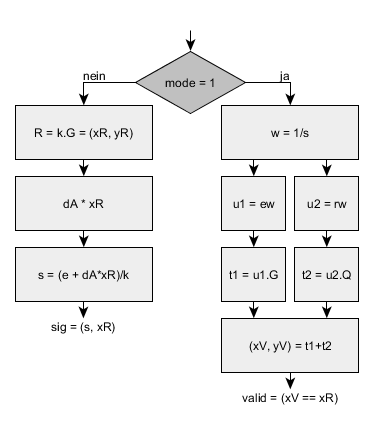
\includegraphics[width=0.6\textwidth]{bilder/vhdl_ecdsa.png}
	\caption{Vereinfachter Ablauf des ECDSA-Algorithmus}
	\label{fig:vhdl-impl-ecdsa}
\end{figure}

Die Algorithmen sind so umgesetzt, dass jede Operation über eine eigene Entität abgebildet wird. So besteht das Signieren aus 3 Entitäten (1x Punktmultiplikation, 1x Multiplizierer, 1x Dividierer), während die Verifikation aus 6 Entitäten (1x Punktaddition, 2x Punktmultiplikation, 2x Multiplizierer, 1xInverter) besteht. Grund für die Verdopplung liegt in erster Linie an der deutlich einfacheren und übersichtlicheren Implementierung. Der Nachteil dagegen ist, dass der Ressourcenverbrauch deutlich höher ist. Da die eingesetzte Hardware aber genügend Ressourcen zur Verfügung stellt, wurde auf eine Optimierung verzichtet. Ein weiterer Vorteil dieser Implementierung ist, dass theoretisch parallel signiert und verifiziert werden kann, was bei einer gemeinsamen Nutzung von Entitäten aufgrund der Umschaltlogik nicht möglich wäre. Für die zeitliche Aktivierung der Entitäten wird wieder auf den Zustandsautomat zurückgegriffen, der die in Abschnitt \ref{vhdl-impl-general-entity} erwähnten Aktivierungs- bzw. Status-Flags verwendet.
\\ \\
Abschließend sei erwähnt, dass der implementierte Algorithmus kleinere Teilkomponenten der Originalfassung nicht berücksichtigt. So wird auf die Überprüfung von Zwischenergebnissen verzichtet. Grund hierfür liegt im wesentlichen an der Tatsache, dass eine ungünstige Wahl der Zufallszahl zu Fehlern führen kann. Da diese Implementierung eine günstige Konstante verwendet, wurde auf ein Abfragen verzichtet. Durch die gewählte Struktur lassen sich  solche Abfragen aber mit wenig Aufwand einbauen, da lediglich der Zustandsautomat angepasst werden muss. Das gleiche gilt für ein nachträgliches Hinzufügen der Zufallszahlgenerierung. \\

\begin{table} [h]
	\centering 
	\begin{tabular}{ | p{3cm} | p{12cm} | }
		\hline
		\textbf{Parameter} & \textbf{Beschreibung}\\
		\hline
		clk\_i & Globales Taktsignal \\
		\hline
		rst\_i & Resetsignal \\
		\hline
		enable\_i & Flag zum Aktivieren der Berechnung \\
		\hline
		mode\_i & Flag zum Umschalten zwischen Signieren und Verifizieren \\
		\hline
		hash\_i & Eingabe Text \\
		\hline
		r\_i & R-Komponente der zu verifizierenden Signatur \\
		\hline
		s\_i & S-Komponente der zu verifizierenden Signatur \\
		\hline
		ready\_o & Status-Flag ob die Berechnung abgeschlossen ist  \\
		\hline
		valid\_o & Flag ob die zu verifizierenden Signatur valide ist \\
		\hline
		r\_o & R-Komponente der erstellten Signatur \\
		\hline
		s\_s & S-Komponente der erstellten Signatur \\
		\hline
	\end{tabular}
	\caption{Eingabe- und Ausgabeparameter der ECDSA-Entität}
	\label{tab:vhdl-impl-ecdsa-param}
\end{table}

\subsection{Punktaddition und -dopplung}
Die Punktaddition und Punktdopplung basieren auf den Formeln aus Abschnitt \ref{sec:ell}. \\

\begin{table} [h]
	\centering 
	\begin{tabular}{ | p{3cm} | p{12cm} | }
		\hline
		\textbf{Parameter} & \textbf{Beschreibung}\\
		\hline
		clk\_i & Globales Taktsignal \\
		\hline
		rst\_i & Resetsignal \\
		\hline
		enable\_i & Flag zum Aktivieren der Berechnung \\
		\hline
		x1\_i & x Komponente des Basis-Punktes \\
		\hline
		y1\_i & y Komponente des Basis-Punktes \\
		\hline
		x2\_o & x Komponenten der Punktdopplung \\
		\hline
		y2\_o & y Komponenten der Punktdopplung \\
		\hline
		ready\_o & Status-Flag ob die Berechnung abgeschlossen ist  \\
		\hline
		\hline
	\end{tabular}
	\caption{Eingabe- und Ausgabeparameter der Punktdopplungs-Entität}
	\label{tab:vhdl-impl-eccdouble-param}
\end{table}

Der zugrundeliegende Ablauf ist identisch mit der Implementierung des ECDSA-Algorithmus, wobei sich lediglich die Formeln unterscheiden. So wird für jede mathematische Operation eine separate VHDL Entität verwendet, die sequentiell über die Aktivierungs- bzw. Status-Flags abgearbeitet werden. Die Umschaltung findet wieder über einen Zustandsautomat statt.

\begin{figure}[thb]
	\centering
	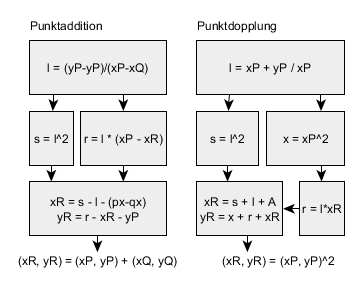
\includegraphics[width=0.7\textwidth]{bilder/vhdl_pa_pd.png}
	\caption{Vereinfachter Ablauf des Punktaddition und -dopplung}
	\label{fig:vhdl-impl-pa-pd}
\end{figure}

Abbildung \ref{fig:vhdl-impl-pa-pd} zeigt den vereinfachten Ablauf der Berechnung. Wie bereits beim ECDSA-Algorithmus wird auch hier ein maximaler Parallelisierungsgrad angestrebt. \\

\begin{table} [h]
	\centering 
	\begin{tabular}{ | p{3cm} | p{12cm} | }
		\hline
		\textbf{Parameter} & \textbf{Beschreibung}\\
		\hline
		clk\_i & Globales Taktsignal \\
		\hline
		rst\_i & Resetsignal \\
		\hline
		enable\_i & Flag zum Aktivieren der Berechnung \\
		\hline
		x1\_i & x Komponente des ersten Punktes \\
		\hline
		y1\_i & y Komponente des ersten Punktes \\
		\hline
		x2\_i & x Komponente des zweiten Punktes \\
		\hline
		y2\_i & y Komponente des zweiten Punktes \\
		\hline
		x3\_o & x Komponenten des Additionsergebnisses \\
		\hline
		y3\_o & y Komponenten des Additionsergebnisses \\
		\hline
		ready\_o & Status-Flag ob die Berechnung abgeschlossen ist  \\
		\hline
		\hline
	\end{tabular}
	\caption{Eingabe- und Ausgabeparameter der Punktadditions-Entität}
	\label{tab:vhdl-impl-eccadd-param}
\end{table}

\subsection{Punktmultiplikation}
Die Punktmultiplikation basiert auf dem Double-And-Add-Algorithmus, der die Zeit für die Berechnung deutlich verkürzt. Der Pseudocode ist in Listing \ref{lst-pm-algo} zu finden.  \\

\begin{lstlisting}[language=Python,frame=single,label=lst-pm-algo,caption=Pseudocode des Double-And-Add Algorithmus]
N = P; Q = 0

for i from 0 to m do
  if di = 1 then
    Q = point_add(Q, N)
  N = point_double(N)

return Q
\end{lstlisting}

Würde anstatt des Double-And-Add-Algorithmus der triviale Algorithmus verwendet werden, so würden für $m = 100 P$ $100$ Punktadditionen benötigt werden, um das Ergebnis zu erhalten. Durch den Einsatz des Double-And-Add-Algorithmus lässt sich die Gleichung umschreiben als $m = 2(2[P + 2(2[2(P + 2P)])])$. Dadurch werden lediglich 6 Punktdopplungen und nur noch 2 Punktadditionen benötigt. \\

\begin{table} [h]
	\centering 
	\begin{tabular}{ | p{3cm} | p{12cm} | }
		\hline
		\textbf{Parameter} & \textbf{Beschreibung}\\
		\hline
		clk\_i & Globales Taktsignal \\
		\hline
		rst\_i & Resetsignal \\
		\hline
		enable\_i & Flag zum Aktivieren der Berechnung \\
		\hline
		xp\_i & x Komponente des Basis-Punktes \\
		\hline
		yp\_i & y Komponente des Basis-Punktes \\
		\hline
		k\_i & Multiplikations-Faktor \\
		\hline
		xq\_o & x Komponenten des Ergebnis-Punktes \\
		\hline
		yq\_o & y Komponenten des Ergebnis-Punktes \\
		\hline
		ready\_o & Status-Flag ob die Berechnung abgeschlossen ist  \\
		\hline
		\hline
	\end{tabular}
	\caption{Eingabe- und Ausgabeparameter der Punktmultiplikations-Entität}
	\label{tab:vhdl-impl-eccmul-param}
\end{table}

\subsection{Polynomreduktion}
Berechnungen wie die Multiplikation führen zu einem Polynom mit einen Grad von $2m-2$, sodass eine Reduktion auf eine Breite von $m$ durchgeführt werden muss.
\\ \\
Für die Reduktion wird eine allgemeine Variante eingesetzt, die eine Nachschlagetabelle anhand des Modulo-Wertes erstellt. Anhand dieser Tabelle wird anschließend ein Eingangspolynom durch Bitverschiebungen, Bitprüfungen und Additionen reduziert.

\subsection{Multiplizierer und Dividierer}
Die Multiplizierer-Entität basiert auf einer klassischen Polynom-Multiplikation, die eine Reihe von Bitverschiebungen, XOR-Verknüpfungen und Polynomreduktionen verwendet. \\

\begin{table} [h]
	\centering 
	\begin{tabular}{ | p{3cm} | p{12cm} | }
		\hline
		\textbf{Parameter} & \textbf{Beschreibung}\\
		\hline
		clk\_i & Globales Taktsignal \\
		\hline
		rst\_i & Resetsignal \\
		\hline
		enable\_i & Flag zum Aktivieren der Berechnung \\
		\hline
		a\_i & Eingabewert 1 \\
		\hline
		b\_i & Eingabewert 2 \\
		\hline
		z\_o & $z = a*b \mod p$ in $GF(2^M)$ \\
		\hline
		ready\_o & Status-Flag ob die Berechnung abgeschlossen ist  \\
		\hline
		\hline
	\end{tabular}
	\caption{Eingabe- und Ausgabeparameter der Multiplizierer-Entität}
	\label{tab:vhdl-impl-mult-param}
\end{table}

Für den Dividierer wurden zwei verschiedenen Implementierungen verwendet, um Laufzeitunterschiede zu messen. Die erste Variante basiert auf einer klassischen Polynomdivision, während die zweite Implementierung eine Multiplikation mit dem Inversen durchführt. \\

\begin{table} [h]
	\centering 
	\begin{tabular}{ | p{3cm} | p{12cm} | }
		\hline
		\textbf{Parameter} & \textbf{Beschreibung}\\
		\hline
		clk\_i & Globales Taktsignal \\
		\hline
		rst\_i & Resetsignal \\
		\hline
		enable\_i & Flag zum Aktivieren der Berechnung \\
		\hline
		g\_i & Eingabewert 1 \\
		\hline
		h\_i & Eingabewert 2 \\
		\hline
		z\_o & $z = g/h \mod p$ in $GF(2^M)$ \\
		\hline
		ready\_o & Status-Flag ob die Berechnung abgeschlossen ist  \\
		\hline
		\hline
	\end{tabular}
	\caption{Eingabe- und Ausgabeparameter der Dividierer-Entität}
	\label{tab:vhdl-impl-divider-param}
\end{table}

\subsection{Quadrier}
Der Quadrierer verwendet eine optimierte Implementierung für Polynome, sodass keine klassische Multiplikation verwendet werden muss. Nach der Bestimmung des Qadradats findet anschließend eine Polynomreduktion statt. 

\begin{table} [h]
	\centering 
	\begin{tabular}{ | p{3cm} | p{12cm} | }
		\hline
		\textbf{Parameter} & \textbf{Beschreibung}\\
		\hline
		clk\_i & Globales Taktsignal \\
		\hline
		rst\_i & Resetsignal \\
		\hline
		enable\_i & Flag zum Aktivieren der Berechnung \\
		\hline
		d\_i & Eingabewert, von welchem das Quadrat gebildet wird \\
		\hline
		c\_o & $c = d^2 \mod p$ in $GF(2^M)$ \\
		\hline
		ready\_o & Status-Flag ob die Berechnung abgeschlossen ist  \\
		\hline
		\hline
	\end{tabular}
	\caption{Eingabe- und Ausgabeparameter der Quadrierer-Entität}
	\label{tab:vhdl-impl-squarer-param}
\end{table}

\subsection{Inverter}
Zum Bestimmen des Inversen wird der erweiterte euklidische Algorithmus eingesetzt. Der Algorithmus bedient sich der Tatsache, dass wenn der Algorithmus das Tripel $d = ggt(a, b), s, t$ ermittelt, ist entweder $d=1$ und damit $1 = t*b \mod a$, sodass $t$ das multiplikative Inverse von $b \mod a$ ist, oder es gilt $d \neq 1$, was bedeutet, dass $b \mod a$ kein Inverses hat. \\

\begin{table} [h]
	\centering 
	\begin{tabular}{ | p{3cm} | p{12cm} | }
		\hline
		\textbf{Parameter} & \textbf{Beschreibung}\\
		\hline
		clk\_i & Globales Taktsignal \\
		\hline
		rst\_i & Resetsignal \\
		\hline
		enable\_i & Flag zum Aktivieren der Berechnung \\
		\hline
		a\_i & Eingabewert, von welchem das Inverse gebildet wird \\
		\hline
		z\_o & $z = 1/x \mod p$ in $GF(2^M)$ \\
		\hline
		ready\_o & Status-Flag ob die Berechnung abgeschlossen ist  \\
		\hline
		\hline
	\end{tabular}
	\caption{Eingabe- und Ausgabeparameter der Inverter-Entität}
	\label{tab:vhdl-impl-inverter-param}
\end{table}

\subsection{Addierer / Subtrahierer}
Die Addition bzw. Subtraktion ist im $GF(2^M)$ trivial, da $-1 = 1$ gilt. Somit muss lediglich eine XOR-Verknüpfung der Operanden durchgeführt werden .  Aufgrund der Einfachheit wurde auf eine separate Entität verzichtet.

\subsection{Test- und Verifizierung}
Für den Test- und die Verifizierung der Entities werden zwei verschiedene Arten von Testbenches verwendet. Die triviale Variante dient lediglich dem kurzen Funktionstest der Entität. Dazu werden lediglich einige statische Werte und Randbedingungen abgefragt, um die Entwicklung der Entitäten zu unterstützen. Die ``echten'' Testbenches dagegen versuchen anhand dynamisch generierter Testdaten die Kombination verschiedener Entitäten zu verifizieren.
\\ \\
Der Tabelle \ref{tab:vhdl-impl-testbenches} ist zu entnehmen, dass beispielsweise die Punktmultiplikation neben der eigentlichen Multiplikation auch die Punktaddition und damit auch die dafür notwendigen mathematischen Grundoperatoren verifiziert. Da es die Testbench erfordert, dass verschiedene Entitäten separat entwickelt werden, was im Fehlerfall die Identifizierung deutlich erschwert, wurden weitere einfachere Testbenches geschrieben, um zunächst die Basisfunktionalität der Entitäten zu verifizieren.
\\ \\
Neben dem reinen Überprüfen der Bedingungen wird teilweise zusätzlich überprüft, ob die Berechnung in einer definierten Anzahl von Taktzyklen abgeschlossen wurde.

\begin{table} [h]
	\centering 
	\begin{tabular}{ | p{5cm} | p{2cm} | p{8cm} | }
		\hline
		\textbf{Beschreibung} & \textbf{Typ} & \textbf{Bedingung}\\
		\hline
		tb\_ecdsa &  dynamisch & \parbox[t]{5cm}{$(r,s)=sign(m)$\\$verify((r,s),m)=True$}  \\
		\hline
		tb\_gf2m\_multiplier & statisch & $a * b = CONST$ \\
		\hline
		tb\_gf2m\_squarer & statisch & $ a * a = CONST$ \\
		\hline
		tb\_gf2m\_eea\_inversion & dynamisch & $x * x^-1 = 1$ \\
		\hline
		tb\_gf2m\_divider & dynamisch & \parbox[t]{5cm}{$c=a/b$\\$c*b=a$} \\
		\hline
		tb\_gf2m\_point\_addition & statisch & $P+Q = CONST $ \\
		\hline
		tb\_gf2m\_point\_doubling & statisch & $P+P = CONST$ \\
		\hline
		tb\_gf2m\_point\_multiplication & dynamisch & \parbox[t]{10cm}{$k.P = (k-1).P + P$\\$k.P = (n-1).P = -P = (xP, xP+yP)$} \\
		\hline
	\end{tabular}
	\caption{Beschreibung der Testbenches}
	\label{tab:vhdl-impl-testbenches}
\end{table}

%%%%%%%%%%%%%%%%%%%%%%%%%%%%%%%%%%%%%%%%%%%%%%%%%%%%%%%%%%%%%
\section{Kommunikation der UART-Verbindung} \label{sec:uartimpl}

Die UART-Komponenten übernehmen wie in Kap. \ref{sec:iuart} beschrieben neben der externen Kommunikation auch die Transformation der Daten. Dabei wird der Rx-Input nach dem Empfangen über die RS232-Schnittstelle auf dem Board\footnote{Das Rx-Signal wird erst nach Einsynchronisation mit zwei aufeinanderfolgenden Flip-Flops verarbeitet.} nach der Verarbeitung über Register mit einem Parallel-Ausgang zur Verfügung gestellt. Abbildung \ref{fig:uartrx} zeigt die Verschaltung des \textit{Receivers} mit den Schieberegistern im RTL Viewer der Entwicklungsumgebung. \\

\begin{figure}[thb]
	\centering
  	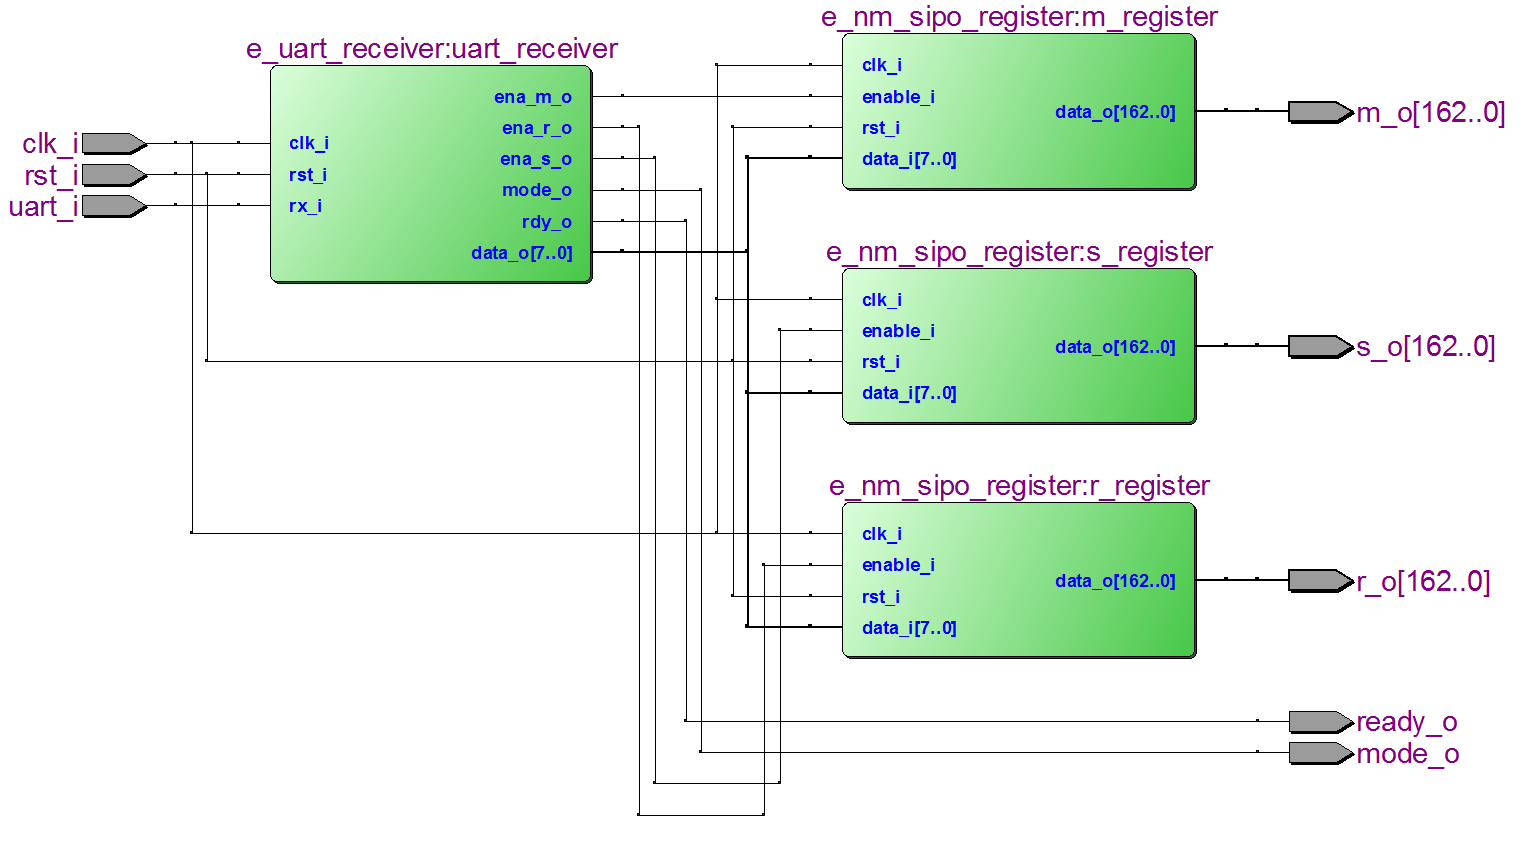
\includegraphics[width=0.9\textwidth]{bilder/uart-receiver}
	\caption{Ansicht des UART-Receivers im RTL Viewer}
	\label{fig:uartrx}
\end{figure}

Der Receiver selbst enthält einen Zustandsautomaten, der den Eingabedatenstrom in die zwei Modi \texttt{Signieren} und \texttt{Verifizieren} klassifiziert. Anhand der Zustände werden die Steuerungssignale am Modulausgang (\textit{enable}-Signale für die Punkte $r$ und $s$ auf der elliptischen Kurve sowie die Nachricht) so geschaltet, sodass jeweils die entsprechenden Eingabewörter in den dafür vorgesehenen Registern landen\footnote{phase1 = $r$, phase2 = $s$, phase3 = $message$} (vgl. Abb. \ref{fig:uart-receiver-phase}). Hierfür gibt es zwei vorangegangene Phase, in denen der Modus durch das erste empfangene Byte bestimmt wird (\textit{dmode}) und anschließend über die Dauer eines Taktzyklus umgeschaltet wird (\textit{smode}). \\

\begin{figure}[thb]
	\centering
  	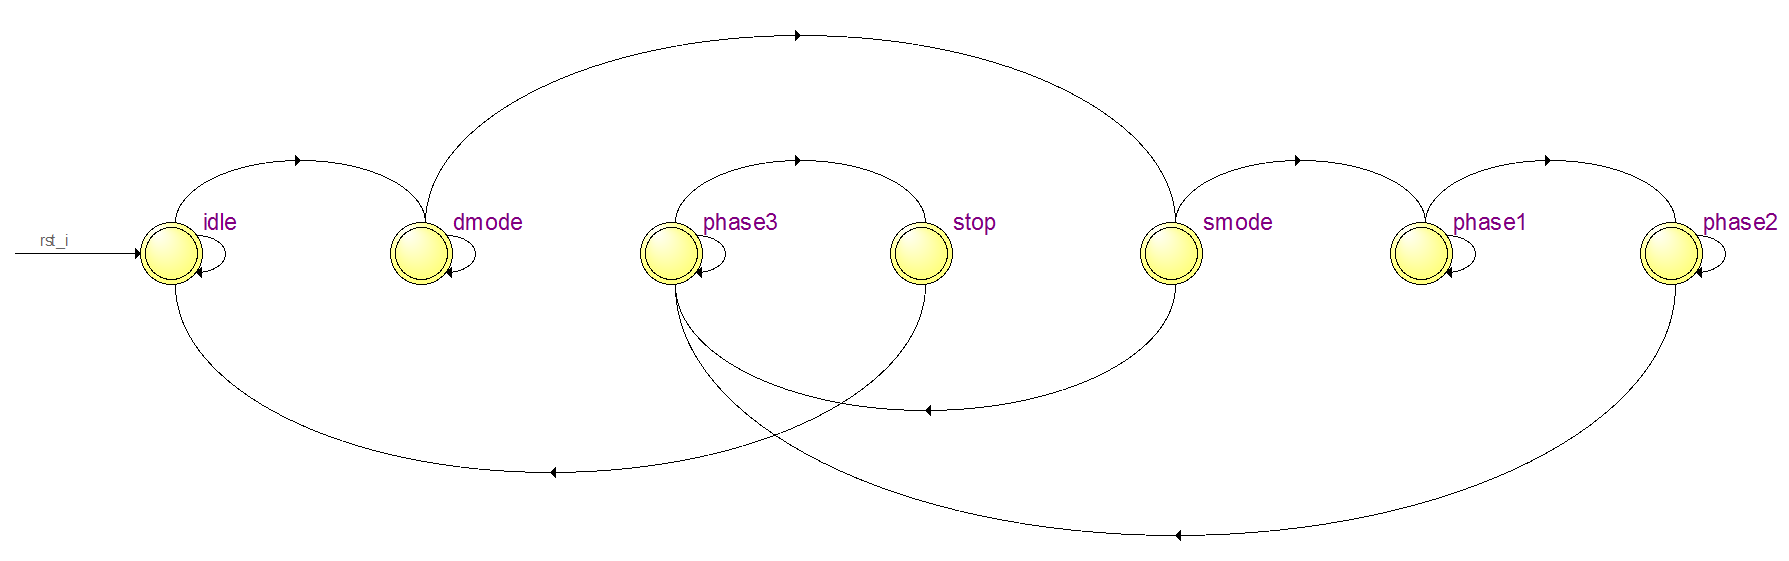
\includegraphics[width=\textwidth]{bilder/uart-receiver-phase}
	\caption{Zustandsautomat des Receivers zu Phasen-Bestimmung beim Empfang}
	\label{fig:uart-receiver-phase}
\end{figure}

Die Phasen des gezeigten Automaten bilden eine Abstraktionsebene über der eigentlichen Erkennung der sequentiellen Datenbits am Rx-Eingang. Ein weiterer Zustandsautomat (s. Anhang \ref{fig:uart-receiver-data}) agiert innerhalb eines UART-Datenpaketes (Start-Bit, 8 Bit Daten, Stop-Bit) und speichert ein einzelnes Byte zwischen zur Weiterverarbeitung. Das erste Byte für den Modus muss dabei entweder ``00000000b'' für das Signieren oder ``11111111b'' für das Verifizieren sein. Der Modus wird als binäres Signal \texttt{mode\_o} vom Receiver-Modul für nachfolgende Module nach außen geführt. \\

Der UART-\textit{Transmitter} beinhaltet zwei Schieberegister, die einen parallelen Eingang mit einem Byte-weise seriellen Ausgang besitzen (vgl. Abb. \ref{fig:uarttx}). Das \texttt{e\_uart\_transmit}-Modul steuert diese Register über einen internen Zustandsautomaten gibt die entsprechenden Steuerungssignale nach außen an die beiden Multiplexer, welche die \textit{enable}-Eingänge anspricht. In diesem Modul wird außerdem eine Timer instantiiert, der anhand der im Package \texttt{tld\_ecdsa\_package} eingestellten Baud-Rate ein Taktsignal für die zu sendenden Datenbits generiert.  \\

\begin{figure}[H]
	\centering
  	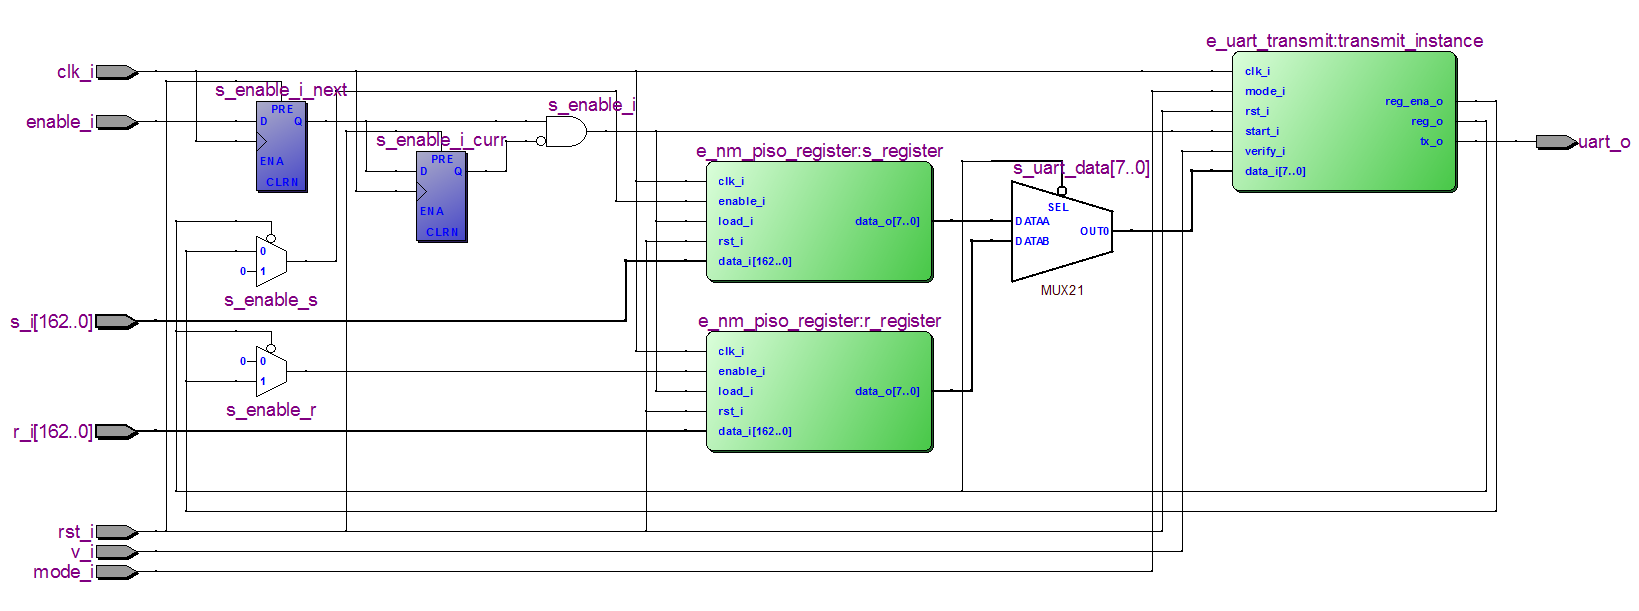
\includegraphics[width=\textwidth]{bilder/uart-transmitter}
	\caption{Ansicht des UART-Transmitter im RTL Viewer}
	\label{fig:uarttx}
\end{figure}

Im Modus Signieren sendet das Modul den in den Registern gespeicherten Punkt $(r, s)$. Beim Verifizieren wird entweder ein Byte Nullen (Signatur passt \textit{nicht} zum Dokument) oder ein Byte Einsen (Signatur gehört zum Dokument) versendet. \\



%%%%%%%%%%%%%%%%%%%%%%%%%%%%%%%%%%%%%%%%%%%%%%%%%%%%%%%%%%%%%
\section{Synthese und Pin-Belegung}

Der verwendete FPGA ist ein Baustein der Altera Cyclone II Familie (EP2C35F672C6). Für die Synthese wird das in der Entwicklungsumgebung Quartus II vom selben Hersteller enthaltene Werkzeug verwendet. \\

Bei der Synthese des entwickelten VHDL-Quellcodes wird vom Synthesewerkzeug zunächst die Netzliste erzeugt. In weiteren Schritten werden Optimierungen auf verschiedenen Ebenen vorgenommen und es findet ein sog. Technology Mapping statt, welche als Basis für die Platzierung und Verdrahtung dienen. Der resultierende Konfigurationskontext kann auf den FPGA übertragen werden. Bei der ECDSA-Entwicklung sind keine Timing-Probleme aufgetreten, die Funktionen und Ergebnisse des Algorithmus beeinflusst haben.
\\ \\

\begin{figure}[H]
	\centering
	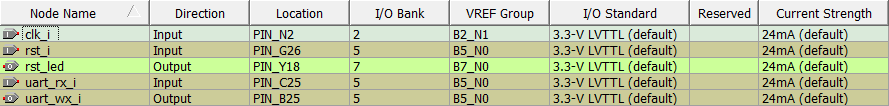
\includegraphics[width=0.8\textwidth]{bilder/pins}
	\caption{Pin-Zuordnung des FPGA}
	\label{fig:pins}
\end{figure}

Abbildung \ref{fig:pins} zeigt die Belegung der verwendeten Pins des Altera DE2 Boards. Um die Testphasen zwischen den einzelnen Synthese-Vorgängen zur Entwicklungszeit abzusichern, wird die Eingabe des auf einen Taster gelegten Reset-Signaleingangs direkt wieder über eine LED-Leuchte nach außen angezeigt. 
\\ \\

\begin{table} [h]
	\centering 
	\begin{tabular}{ | p{5cm} | p{5cm} | }
		\hline
		\textbf{Beschreibung} & \textbf{Wert}\\
		\hline
		Ressourcennutzung & 21\% \\
		\hline
		Anzahl Logikelemente & 23,781 / 33,216 ( 72 \% ) \\
		\hline
		Anzahl Register & 15508 \\
		\hline
		Anzahl Pins & 5 / 475 ( 1 \% ) \\
		\hline
	\end{tabular}
	\caption{Ergebnisse der Synthese}
	\label{tab:vhdl-impl-de2}
\end{table}

Das Report des Synthesewerkzeugs nennt eine Auslastung der Logikelemente um 72\% und eine Gesamtressourcennutzung um 21\%. 
\\ \\


